\subsection{基本硬布线控制器}

TEC-8各个部件控制信号可以看做是硬布线控制器输入的组合逻辑,使用Verilog HDL可以控制硬布线控制器按照一定的逻辑输出控制信号以
实现顺序硬布线控制器。组合逻辑可以由控制器的流程图看出,经过小组讨论,我们选择了如下的流程图\ref{fig:basic_flowchart}作为实现硬布线控制器的参考流程图

\begin{figure}[htbp]
    \centering
    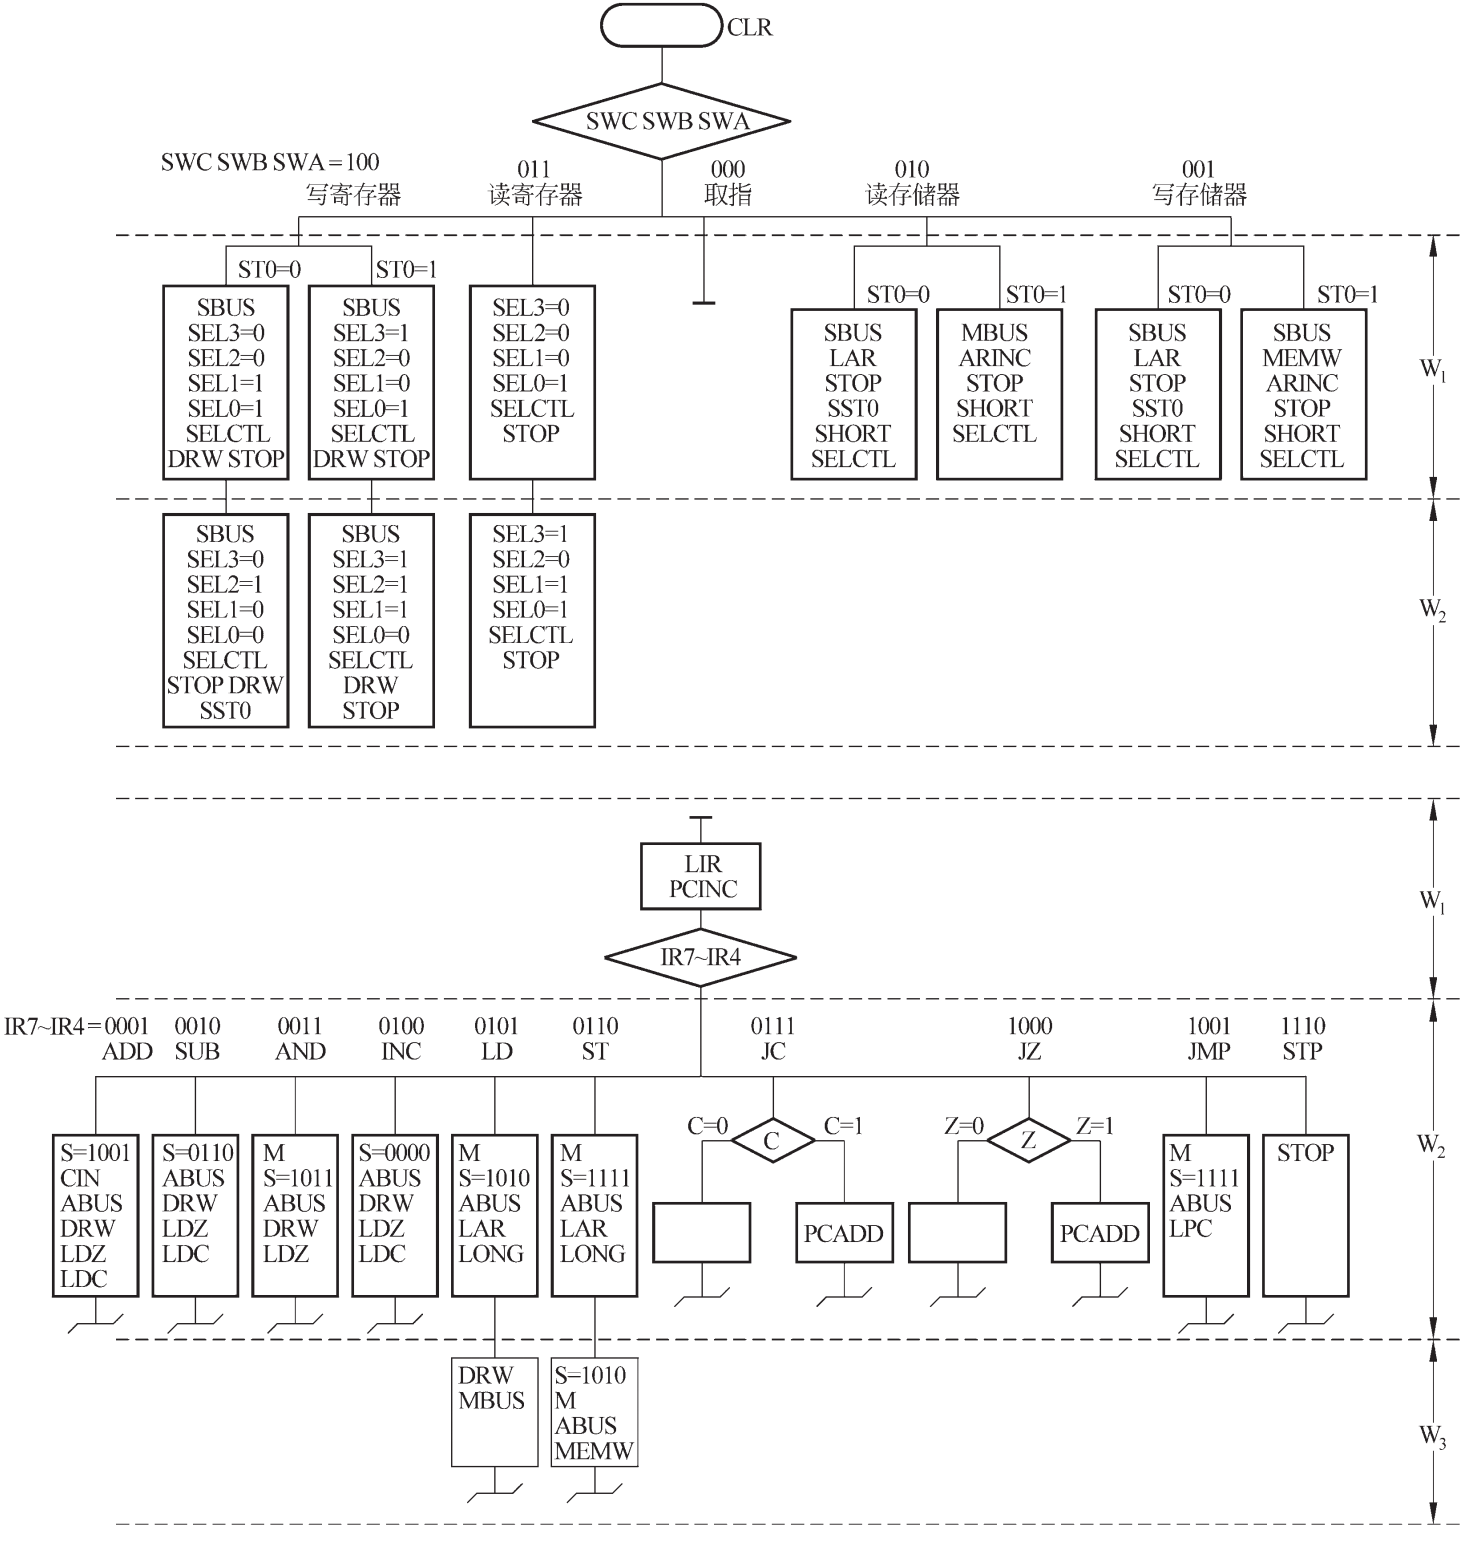
\includegraphics[width=0.8\linewidth]{figures/chapter2/basic_flowchart.png}
    \caption{基本硬布线控制器流程图}
    \label{fig:basic_flowchart}
\end{figure}

由上图可以看出每一个控制信号是否置1可以由控制台模式选择SWCBA、阶段标志ST0、节拍脉冲W1\~{}3、IR7\~{}4决定,按照流程图可以写出
每个信号的组合逻辑,便可以实现基本的硬布线控制器。

控制台操作包括写寄存器、读寄存器、读存储器、写存储器。写寄存器时SELCTL置1,通过SEL3 SEL2选中寄存器。
SBUS置1让数据开关数据进入DBUS,DRW置1使得T3上升沿到来时DBUS数据写入选中的寄存器。写寄存器功能需要能写四个
寄存器,故设计时考虑SEL3 SEL2轮流选择R0\~{}R3,依次写入数据。

\subsubsection{写寄存器}
写入哪个寄存器有节拍电位信号来决定,由于时序发生器最多产生三个节拍W1\~{}W3,故无法满足四个节拍分别对应写四个寄存器。
因此在设计写寄存器时,采用一个标志变量ST0来判断目前写寄存器的阶段。当ST0为0时,W1,W2节拍分别写入R0,R1。在ST0为1时
W1,W2两个节拍分别写入R2,R3。

\subsubsection{读寄存器}
在读寄存器时,由于TEC-8可以显示如图\ref{fig:construction_of_tec8}中两个四选一选择器A和B的输出值,故读寄存器
可以一次读两个寄存器的值,故读寄存器只需要两个节拍W1 W2即可。

读寄存器时SEL3 SEL2控制选择器A,SEL1 SEL0控制选择器B,在不同节拍设置不同值即可分别读出四个寄存器的值。

\subsubsection{读存储器}
读存储器分为两个阶段,第一个阶段由用户输入指定地址,第二个阶段从该输入地址依次读出一个字节的值。

存储器读出值时地址由AR指定,故读入地址时LAR置1,数据由数据开关得到,故SBUS为1,由于该阶段可以由一个节拍完成,
故不需要输出节拍信号W2,因此此时SHORT输出应为1以使时序发生器不产生W2节拍。

读入地址后,接着将依次读出数据,为了和读入地址阶段进行区分,程序使用ST0=1来标识第二阶段。第二阶段需要将MBUS置1
以使存储器AR地址处的值通过DBUS输出,为实现连续地址读取,需将ARINC置1,使得下一个节拍时地址加一。

\subsubsection{写存储器}
写存储器流程与读存储器流程基本一致,由流程图\ref{fig:basic_flowchart}可以编写输出信号逻辑。

\subsubsection{取指执行}
要实现的基本指令如图\ref{fig:instruction}所示。

对于运算指令、跳转指令和停机指令,我们采用两个节拍电位来完成取指和执行操作,其中W1节拍用于取指,该节拍时LIR PCINC有效,以实现
将PC对应地址处指令取出并写入指令寄存器IR;在W2节拍,根据取出指令类型(即IR7\~{}IR4)来输出不同的控制信号。

对于存取指令(LD和ST),需要使用三个节拍来完成指令,其中W1时取指令,W2时将期望的地址写入AR寄存器,W3节拍时将数据从寄存器写入存储器或将数据读出到寄存器。
在默认情况下时序发生器只产生两个节拍电位W1和W2,故在程序设计时需要在这两条指令的W2阶段输出Long信号使时序发生器产生W3节拍电位信号。

\subsubsection{执行程序前指定PC值}
为了能区分当前处于修改PC阶段还是取指执行阶段,我们还是采用状态变量ST0进行标志,当ST0为0时,由用户通过数据开关输入PC,此时
LPC SBUS置1,由于该操作只需要一个节拍电位即可完成,故SHORT输出为1,使时序发生器不产生W2节拍。当修改PC完成后,标志ST0置1,
进入正常取指执行阶段。

指定PC的操作对应的修改后的流程图如图\ref{fig:pc_modifier}
\begin{figure}[htbp]
    \centering
    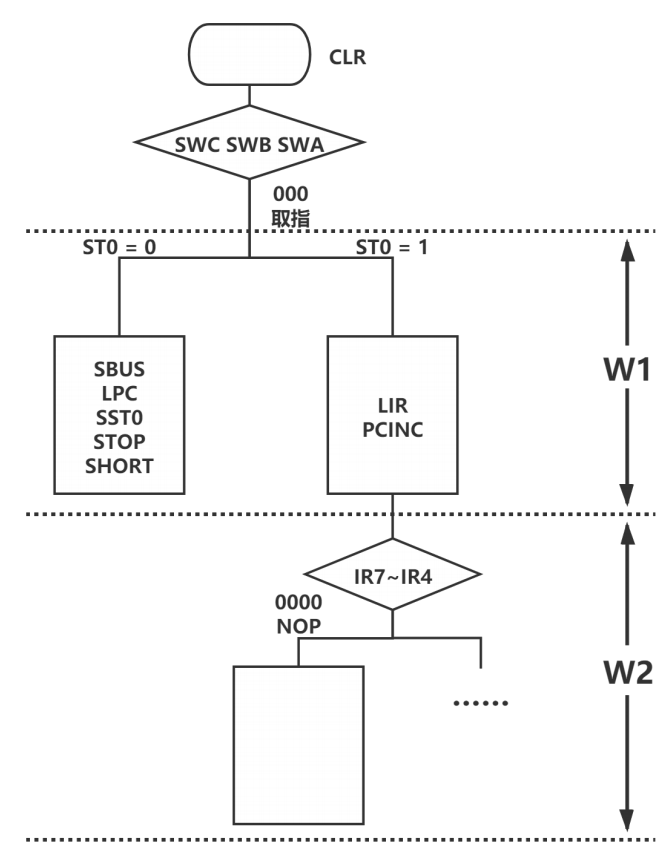
\includegraphics[width=0.7\linewidth]{figures/chapter2/PC_modifier.png}
    \caption{用户指定PC流程图}
    \label{fig:pc_modifier}
\end{figure}

\subsubsection{拓展指令}
IR7\~{}IR4标志着指令类型,四位最多可以支持16条指令,基本指令只有10条,经过小组讨论,我们选择拓展XOR、DEC、STP和NOP指令,总体流程与其他指令一致,输出信号略有不同。

\subsubsection{译码表}
依据流程图编写译码表如图\ref{fig:decoding_table}

\begin{figure}[htbp]
    \centering
    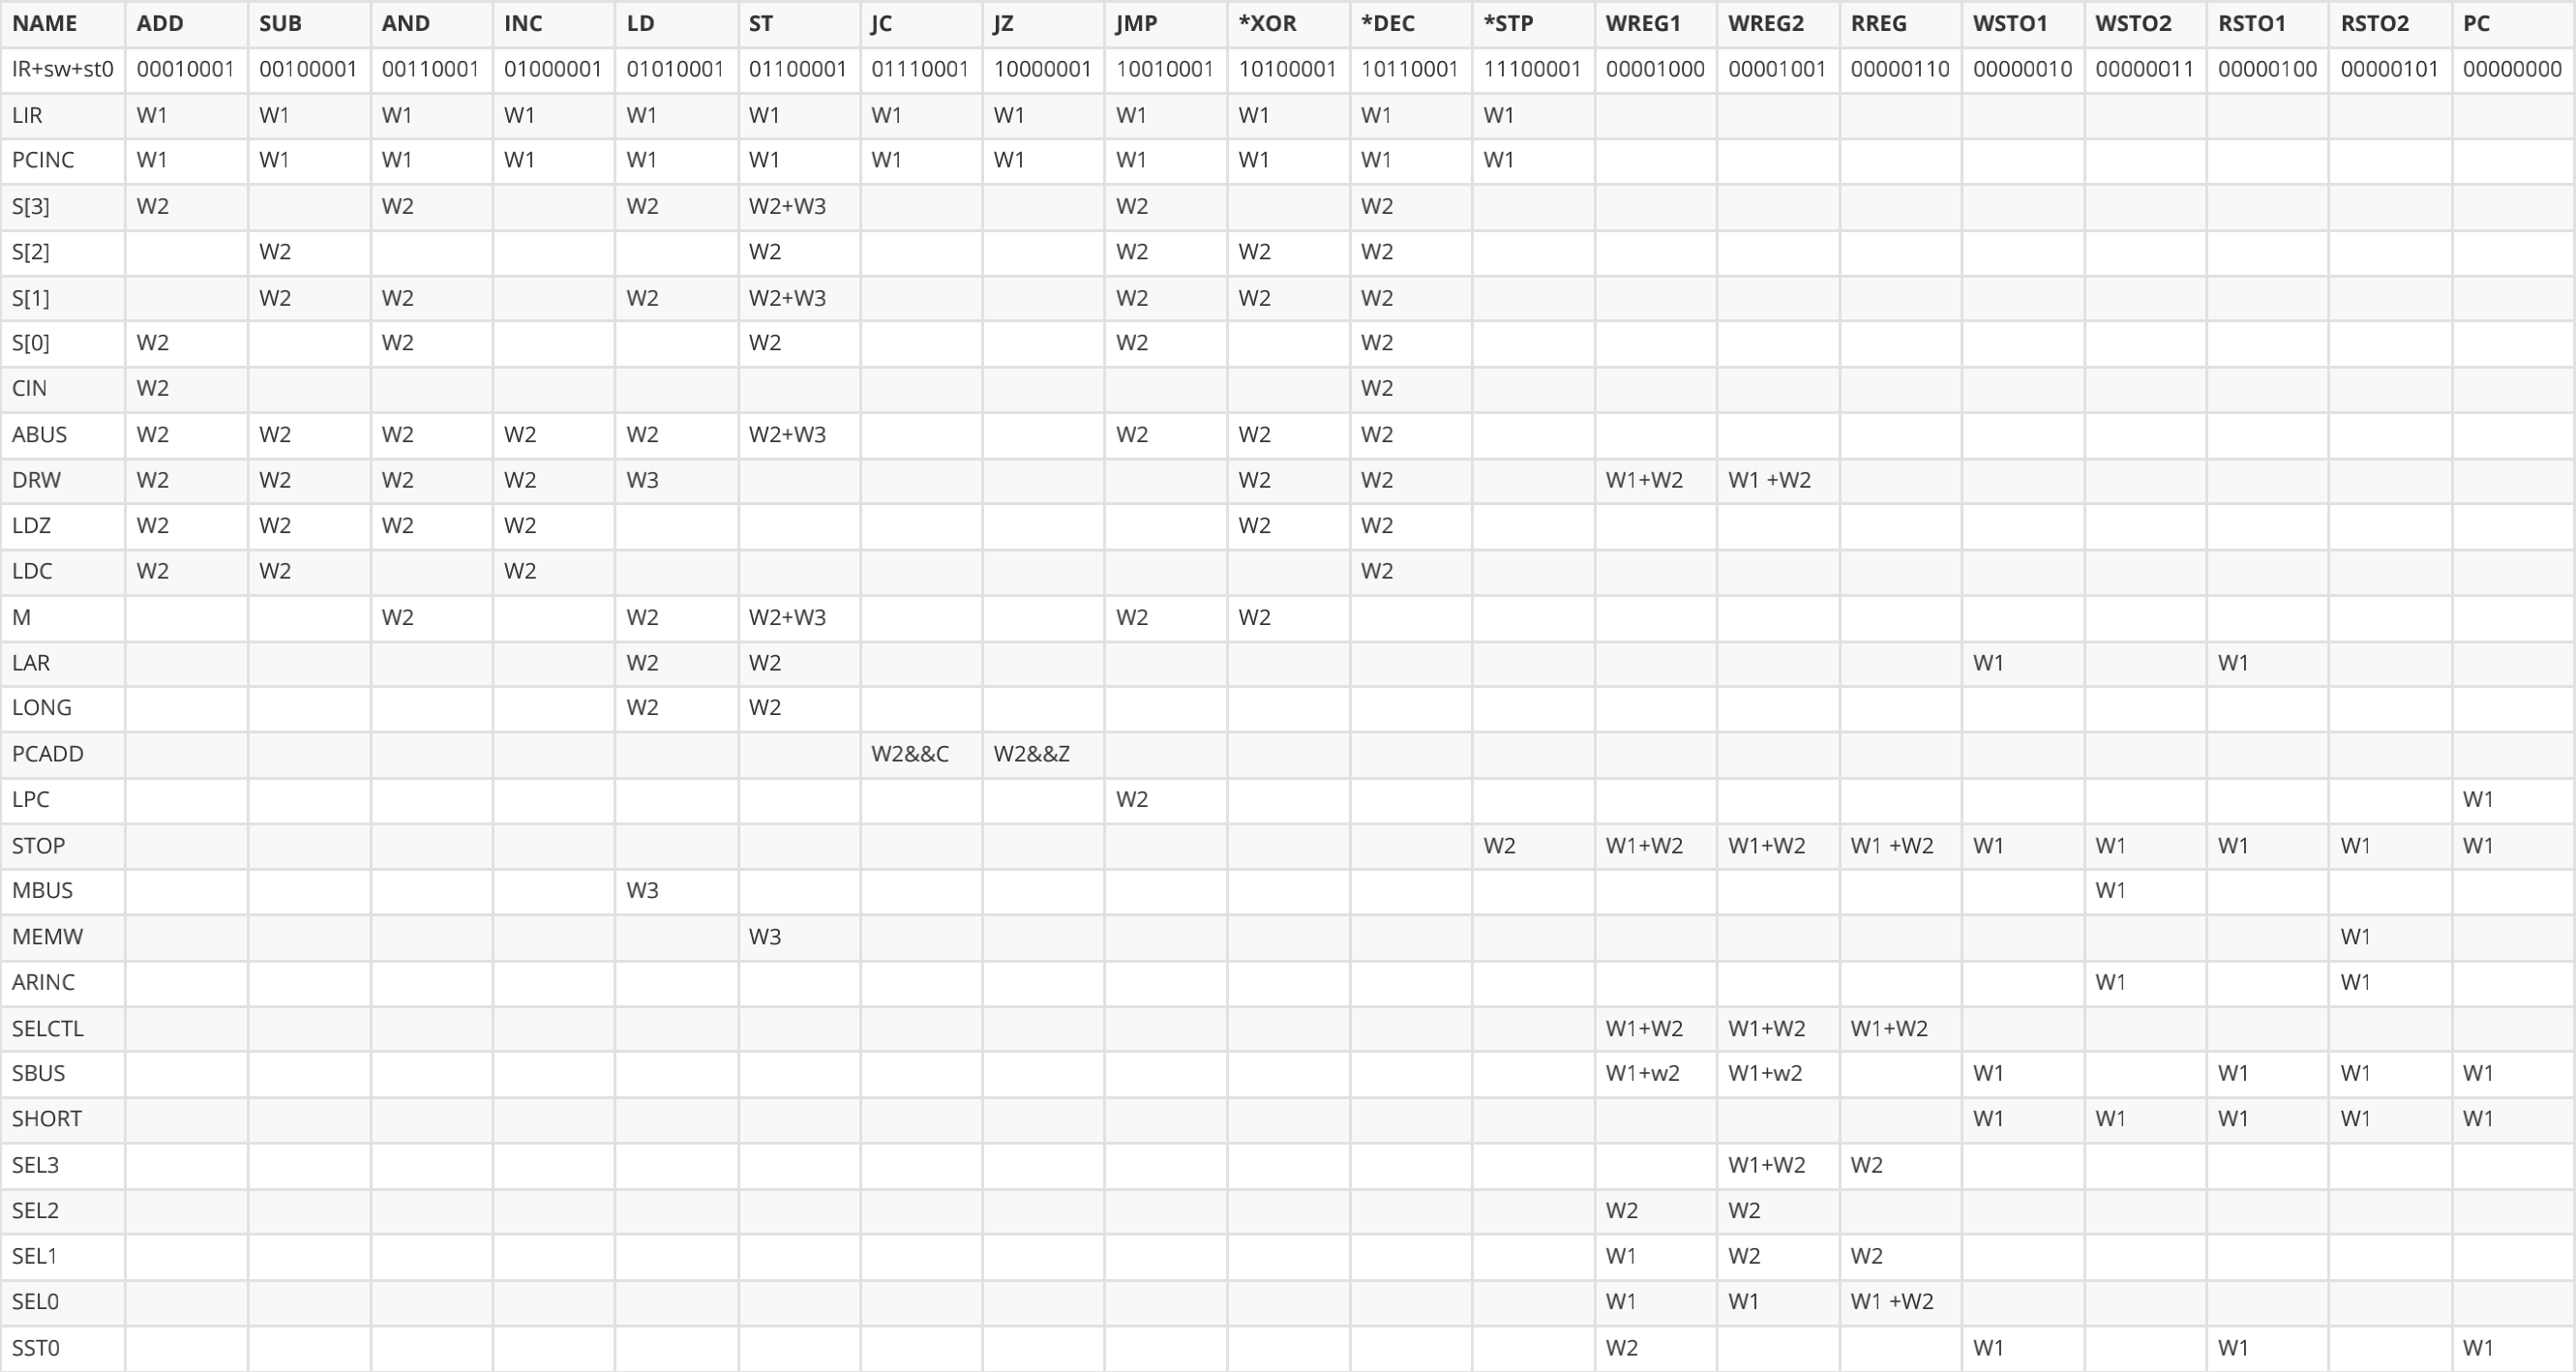
\includegraphics[width=0.9\linewidth]{figures/chapter2/decoding_table.png}
    \caption{基本硬布线控制器译码表}
    \label{fig:decoding_table}
\end{figure}

硬布线控制器代码基于译码表编写。
\clearpage
